\task{Имеется 8~внешне совершенно одинаковых свинцовых шариков, 
однако внутри одного из них сделана небольшая полость. Пользуясь 
только рычажными весами, определите, какой шарик с полостью. Весы 
можно использовать не более двух раз. Опишите свои действия и 
сделайте рисунок.}

\task{Два друга, Петр и Павел, поехали на поезде. У Петра был билет в 
первый вагон, а у Павла --- в последний (вагоны нумеруются от 
локомотива). На одной из промежуточных остановок локомотив 
перецепили к хвосту поезда, поэтому Петр приехал в конечный 
пункт в последнем вагоне, а Павел --- в первом. Сравните пути 
вагонов, в которых ехали Петр и Павел.}

\task{Заводной игрушечный автомобиль едет по полу. В кузове 
автомобиля стоит оловянный солдатик. Автомобиль сталкивается со 
стенкой. В каком направлении по отношению к направлению движения 
автомобиля упадет солдатик? Ответ обоснуйте.}

\task{Имеется чайник с водой, нить, мензурка и тело неправильной 
формы, не входящее в мензурку.  Как можно определить объем этого 
тела? Опишите и сделайте рисунок.}

\task{Эскалатор одной из станций метро поднимает неподвижно 
стоящего на нем пассажира в течение 2~мин. По неподвижному 
эскалатору пассажир поднимается в течение 6~мин. Сколько времени 
будет подниматься пассажир идущий вверх по движущемуся 
эскалатору?}

\task{С лодки, идущей вниз по течению реки, уронили в воду весло. 
Через час после этого решили подобрать весло и повернули 
обратно. Через какое время лодка повстречает весло, если 
скорость течения одинакова по всей реке, а мотор лодки все время 
работает в одинаковом режиме?}

\task{Пеностекло получают вспениванием стекла в процессе варки, 
вводя пенообразующее вещество. Сколько процентов объема 
пеностекла занимают газы, массой которых можно пренебречь, если 
плотность пеностекла $\rho_1 = 200\mbox{ кг/м}^3$? Плотность обычного 
стекла $\rho_0 = 2500\mbox{ кг/м}^3$.}

\taskpic{В изогнутую трубку наливают воду до тех пор, пока она не 
начинает переливаться через край. Широкое колено закрывают 
крышкой массой $M$. Какую массу воды нужно долить, чтобы крышка 
поднялась? Площадь широкого колена $S_1$, площадь узкого колена 
$S_2$.}{
\begin{tikzpicture}
  \draw[thick,fill=blue!20] (3.5,3) -- (3.5,0) -- (0.5,0) --
  (0.5,2) -- (1.5,2) -- (1.5,0.5) -- (3,0.5) -- (3,3);
  \draw[pattern=north east lines] (0.4,2) rectangle ++(1.2,0.3);
  \draw (1,1.7) node {$S_1$};
  \draw (3.25,3.25) node {$S_2$};
\end{tikzpicture}  
}

\task{Идет дождь. Капли падают вертикально со скоростью $v$. 
Неподвижное цилиндрическое ведро с площадью дна $S$ наполняется 
со скоростью 1~кг/мин. Самолет летит горизонтально со скоростью 
$4v$. Какая масса воды попадает за минуту в цилиндрический 
воздухозаборник самолета площадью $2S$?}

\task{Судно выходит из реки в море. Как при этом изменяется 
архимедова сила, действующая на судно? Ответ обоснуйте.}

\task{Оцените массу атмосферы Венеры. Венеру считать шаром с 
площадью поверхности $4{,}7\cdot10^{14}\mbox{ м}^2$. Величина $g$ для Венеры 
равна 8{,}7~Н/кг. Атмосферное давление у поверхности Венеры 9120~кПа.}

\task{Тело подвешено на пружине динамометра. При взвешивании тела в 
пустоте показание динамометра $P$. При взвешивании этого же тела в 
жидкости плотностью $\rho_1$ динамометр показывает $P_1$. Какова 
плотность тела? При взвешивании тело полностью погружается в 
жидкость и не растворяется в ней.}

\task{Катер плывет по реке против течения с постоянной скоростью и 
в некотором определенном месте теряет спасательный круг. Через 
время $t$ потеря обнаруживается, катер поворачивает обратно и 
нагоняет круг на расстоянии $S$ ниже места потери. Какова скорость 
течения реки, если мотор катера при движении против течения и по 
течению работает в одинаковом режиме?}

\task{Тело подвешено на пружине динамометра. При взвешивании тела в 
пустоте показания динамометра $P$. При взвешивании этого же тела в 
жидкости с плотностью $\rho_1$ динамометр показывает $P_1$. При 
взвешивании тела в жидкости с неизвестной плотностью $\rho_2$ 
динамометр показывает $P_2$. Какова плотность жидкости $\rho_2$? При 
взвешивании тело полностью погружается в обе жидкости и не 
растворяется в них.}

\task{Из города А выехала автомашина, движущаяся со скоростью 10~м/с, 
и одновременно навстречу ей из города В выехал велосипедист, 
движущийся со скоростью 18~км/ч. Расстояние между городами 108~км 
(путь прямой). Постройте график зависимости пройденного пути от 
времени для каждой машины и по этим графикам определите 
пройденные пути и время движения автомашины и велосипедиста до 
их встречи.}

\task{В сосуде с водой плавает шар, наполовину погрузившись в воду. 
Изменится ли глубина погружения шара, если этот сосуд с шаром 
перенести на планету, где сила тяжести в два раза больше, чем на 
Земле?}

\task{Мальчик проплыл на надувной лодке по реке вниз и вверх по 
течению, а затем, прилагая те же усилия к той же лодке, проделал 
такой же длины путь по озеру со стоячей водой. В котором случае 
мальчик расходовал меньше времени, проплывая намеченный им путь?}

\task{Ко дну сосуда с водой приморожен шарик из льда. Как изменится 
уровень воды в сосуде, когда лед растает? Изменится ли при этом 
сила давления воды на дно сосуда?}

\task{Для барометра мальчики сделали барометрическую трубку, в 
которой средняя часть (в несколько сантиметров длиной) 
представляет трубку из эластичной резины. Как под действием 
ртути в такой составной трубке их барометра была деформирована 
резиновая часть трубки --- сузилась или расширилась?}

\task{В сосуде с водой плавает кусок льда. Изменится ли уровень воды 
в сосуде, если лед растает?}

\task{Теплоход движется со скоростью 18~км/ч. По его палубе от кормы 
до носовой части и обратно идет пассажир со скоростью 3{,}6~км/ч 
относительно теплохода. Какой путь относительно берега пройдет 
пассажир, если длина теплохода 100~м?}

\task{В сосуде с водой плавает кусок льда, в котором находится 
пузырек воздуха. Изменится ли уровень воды в сосуде, когда лед 
растает?}

\task{Первую треть пути мотоциклист проехал со скоростью 40~км/ч, 
остальной путь --- 50~км/ч. Определите среднюю скорость движения на 
всем пути.}

\task{В сосуде с водой плавает кусок льда с вмерзшим в него стальным 
шариком. Изменится ли уровень воды в сосуде, когда лед растает?}

\task{В цилиндрический сосуд с площадью основания $S = 100\mbox{ см}^2$ 
налит 1~литр соленой воды плотности $\rho_1 = 1{,}15\mbox{ г/см}^3$. В этой 
воде плавает кусок льда из пресной воды массой $m = 1\mbox{ кг}$. 
Определите, как изменится уровень воды в сосуде, если половина 
льда растает. Считать, что при растворении соли в воде объем 
жидкости не изменяется.}

\task{В сосуде с водой на подставках находится цилиндр без дна. 
Высота выступающей из воды части цилиндра равна $h = 5\mbox{ см}$. 
Какую высоту должен иметь цилиндр, чтобы его можно было 
заполнить маслом целиком?}

\task{В сосуде с водой плавает брусок из льда, на котором лежит 
деревянный шар. Плотность вещества шара меньше плотности воды. 
Изменится ли уровень воды в сосуде, если лед растает?}

\task{Вагон поезда, движущегося со скоростью 36~км/ч, был пробит 
пулей, летевшей перпендикулярно к движению поезда. Одно 
отверстие в стенках вагона смещено относительно другого на 3~см. 
Ширина вагона --- 2{,}7~м. Какова скорость движения пули?}

\task{Когда мимо пристани проходил плот, в деревню, находящуюся на 
расстоянии 15~км от пристани, вниз по реке отправилась моторная 
лодка. Она дошла до деревни за $\frac{3}{4}$ часа и, повернув обратно, 
встретила плот на расстоянии 9~км от деревни. Какова скорость 
течения реки и скорость лодки относительно воды?}

\task{На чашке весов стоит стакан с водой. Изменятся ли показания 
весов, если в воду погрузить гирю, подвешенную на нити к штативу?}

\task{Большой круг установлен в центре прямоугольного зала на 
уровне пола и равномерно вращается. Мальчик, часто подпрыгивая 
на одной ноге, пересекает круг в направлении диагонали зала. При 
этом на круге остается след ступни мальчика. Сплошной линией 
покажите траекторию движения мальчика относительно круга. 
Скорость мальчика (относительно земли) считать такой, что за то 
время, пока круг делает половину оборота, мальчик преодолевает 
путь, равный длине диаметра круга.}

\taskpic{На равноплечных весах уравновешены два одинаковых 
цилиндрических сосуда с водой. Уровни воды в обоих сосудах 
совпадают. В сосуд опускают одинаковые шары объема $V$ массы $M$ 
каждый, плотности которых меньше плотности воды. В левый сосуд 
шар опускают на жесткой штанге, к концу которой он привязан с 
помощью нити. В правый сосуд шар опускают на нити, перекинутой 
через неподвижный блок. Оба шара полностью погружены в воду. 
Какой груз и на какую чашку надо добавить, чтобы не нарушилось 
равновесие? Объемами штанги, нити, блока пренебречь. Плотность 
воды считать известной.}{
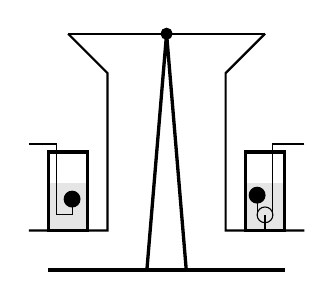
\begin{tikzpicture} 
  \draw[very thick] (0.5,0) -- (3.5,0);
  \draw[very thick] (1.75,0) -- (2,3) -- (2.25,0);
  \draw[fill=black] (2,3) circle (0.07);
  \draw[thick] (0.75,3) -- (3.25,3);
  \draw[thick] (0.75,3) -- (1.25,2.5) -- ++(0,-2) -- ++(-1,0);
  \draw[thick] (3.25,3) -- (2.75,2.5) -- ++(0,-2) -- ++(1,0);
  \draw[fill=gray!20,draw=gray!20] (0.5,0.5) rectangle ++(0.5,0.6);
  \draw[fill=gray!20,draw=gray!20] (3,0.5) rectangle ++(0.5,0.6);
  \draw[very thick] (0.5,0.5) rectangle ++(0.5,1);
  \draw[very thick] (3,0.5) rectangle ++(0.5,1);
  % жёсткая штанга
  \draw (0.25,1.6) -- (0.6,1.6) -- ++(0,-0.9) -- ++(0.2,0) --
  ++(0,0.2);
  \draw[fill=black] (0.8,0.9) circle (0.1);
  % блок в правом сосуде
  \draw (3.25,0.5) -- ++(0,0.2);
  \draw (3.25,0.7) circle (0.1);
  \draw (3.75,1.6) -- (3.35,1.6) -- ++(0,-0.9);
  \draw (3.15,0.7) -- ++(0,0.2);
  \draw[fill=black] (3.15,0.95) circle (0.1);
\end{tikzpicture}  
}

\task{На тренировке по баскетболу два спортсмена выполняют 
передачи мяча, непрерывно двигаясь навстречу друг другу. Сколько 
передач они успеют сделать до того момента, когда пробегут мимо 
друг друга, если скорости движения спортсменов постоянны и равны 
1~м/с, скорость полета мяча --- 10~м/с, время, затрачиваемое на каждый 
прием и передачу --- 0{,}2~с. Начальное расстояние между 
баскетболистами --- 10~м.}

\task{Толстостенная лодка с вертикальными стенками и отверстием в 
дне достаточно долго свободно плавает в озере. Затем отверстие 
затыкают и потом внутрь лодки пускают плавать бревно. Повысится 
или понизится после этого уровень воды в лодке относительно 
уровня воды в озере?}

\task{Наблюдая за равномерно движущимся поездом, мальчик 
определил, что мимо начала железнодорожной платформы поезд 
двигался в течение времени $t_1 = 23\mbox{ c}$. Одновременно с этим его 
приятель установил, что мимо этой платформы поезд двигался в 
течение времени $t_2 = 39\mbox{ c}$. Измерив длину платформы, которая 
оказалась равной $l = 240\mbox{ м}$, мальчики определили скорость и 
длину поезда. Какие числовые значения этих физических величин 
получили мальчики?}

\task{В сосуде с водой плавает железный коробок, ко дну которого при 
помощи нити подвешен стальной шар. Шар не касается дна сосуда. 
Как изменится высота уровня воды в сосуде, если нить, 
удерживающая шар, оборвется?}

%%% Local Variables: 
%%% mode: latex
%%% TeX-master: "../../report"
%%% End: 
